\documentclass[12pt]{article}
\usepackage[a4paper, total={7.5in, 11in}]{geometry}
%\usepackage{array}
\usepackage{graphicx, subfig, wrapfig, fancyhdr, lastpage, multicol ,color,arydshln,makecell, mhchem, multirow}
\newcommand\headerMe[2]{\noindent{}#1\hfill#2}
\usepackage[mathscr]{euscript}
\usepackage{tabularray}

\setlength{\columnseprule}{1pt}
\def\columnseprulecolor{\color{blue}}


\pagestyle{fancy}
\fancyhf{}

\cfoot{ \vspace{-0.8cm}\em{Page \thepage \hspace{1pt} / \pageref{LastPage}}}
\begin{document}

\headerMe{Royaume du Maroc}{année scolaire \emph{2024-2025}}\\
\headerMe{Ministère de l'Éducation nationale, }{  Professeur :\emph{Zakaria Haouzan}}\\
\headerMe{du Préscolaire et des Sports}{Établissement : \emph{Lycée SKHOR qualifiant}}\\
%\vspace{-1cm}
\begin{center}
Devoir Surveillé  N°2 \\
    2ème année baccalauréat Sciences Mathématiques\\
Durée 2h00
\\
    \vspace{.2cm}
\hrulefill
\Large{Chimie 7pts - 45min}
\hrulefill\\

\end{center}
%end Headerss------------------------
%__________________Chimie ______________________-
%%%%%%%+_+_+_+_+_+_+_+_+_Partie1

 \section*{Transformations non totales d'un système chimique\dotfill(7pts)-45min }
%\begin{wrapfigure}{r}{0.16\textwidth}
	%\vspace{-1.2cm}
%%\begin{center}
  %%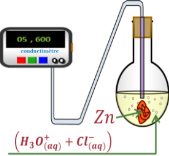
\includegraphics[width=0.16\textwidth]{./img/chimie01.png}
%%\end{center}
%\end{wrapfigure}


%\begin{wrapfigure}[1]{r}{0.5\textwidth}
	%\vspace{0.5cm}
%\begin{center}
  %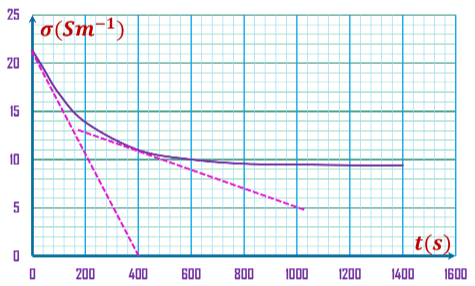
\includegraphics[width=0.5\textwidth]{./img/chimie02.png}
%\end{center}
%\end{wrapfigure}

\textit{L’acide benzoïque $C_6H_5COOH$ (que l’on pourra noter AH) et le benzoate de sodium
$C_6H_5COONa$ (que l’on pourra noter NaA) sont des solides conservateurs alimentaires, utilisés en
particulier dans les boissons rafraîchissantes de type soda ; ils sont respectivement désignés par le code
européen E 210 et E 211. }

Cet exercice a pour objectif de d’étudier le comportement d’acide benzoïque.

Données pour tout l’exercice 
	Les conductivités molaires ioniques : $ \lambda_1= \lambda_{H_3O^+}$=$35.mS.m^2/mol$ ; 

  $\lambda_2= \lambda_{Cl^-}$=$7,63.mS.m^2/mol$; $\lambda_3 = \lambda_{C_6H_5COO^-}$=$3,25.mS.m^2/mol$ ; 

  $\lambda_4= \lambda_{Na^+}$=$5.mS.m^2/mol$ ; $\lambda_5= \lambda_{CH_3COO^-}$=$4,1.mS.m^2/mol$


 \section*{Partie 1 : Étude  pH-métrique d’une solution d’acide benzoïque
}

1.On dispose d’une solution aqueuse $( S_A )$ d’acide benzoïque $C_6H_5COOH$ de concentration molaire en soluté apporté 
$C_A = 1,5.10^{-2} mol.L^{-1}$ . Son pH est égal à 3,0.

	\begin{tabular}{c|l}
		0,25 & \makecell[l]{\textbf{1.1 }Ecrire l’équation de la réaction entre l’acide benzoïque et l’eau. }\\


		0,75 & \makecell[l]{\textbf{1.2 }Exprimer et calculer le taux d’avancement final $\tau$ de cette réaction.}\\

		0,75 & \makecell[l]{\textbf{1.3 }exprimer la constante d’équilibre en fonction de $C_A$ et $\tau$ .calculer sa valeur }\\

    0,75 & \makecell[l]{\textbf{1.4. }Qu’elle sera la valeur du taux d’avancement $\tau'$ pour une solution aqueuse d’acide benzoïque \\de concentration $C_A' = \frac{C_A}{20}$ . justifier}
			
	\end{tabular}

  \vspace{0.4cm}
2.On considère une solution aqueuse d’acide benzoïque $C_6H_5COOH$ de concentration molaire en soluté apporté $C$ et de volume V. la mesure de la conductance de cette solution donne la valeur $G_1 = 8,6.10^{-5}S$ , la conductance d’une solution aqueuse d’acide chlorhydrique  $(H_3O^+ + Cl^-)$ de même concentration et dans les mêmes conditions est $G_2 = 4,3.10^{-4}S$

	\begin{tabular}{c|l}
		0,25 & \makecell[l]{\textbf{2.1. }Dresser le tableau descriptif de l’évolution du système de la réaction entre \\l’acide
benzoïque et l’eau.}\\

		1 & \makecell[l]{\textbf{2.2. }Exprimer le taux d’avancement final $\tau$, de la réaction d’acide benzoïque en fonction \\de $G_1$, $G_2$, $\lambda_{Cl^-}$, $\lambda_{H_3O^+}$, $\lambda_{C_6H_5COO^-}$Calculer sa valeur. }\\


		0,75 & \makecell[l]{\textbf{2.3. }Calculer la concentration molaire $C$ .}\\



	\end{tabular}
	
  \vspace{0.4cm}
3.On mélange dans un becher un volume $V_0 = 50mL$ d’une solution aqueuse d’acide benzoique $C_6H_5COOH$ de concentration $C_0 = 6.10^{-2}mol/L$ avec le même volume $V_0$ d’une solution d’ethanoate sodium\\ $(CH_3COO^-_{(aq)}, Na^+_{(aq)})$, de même concentration $C_0$

La mesure de la conductivité de la solution à l’équilibre a donnée: $\sigma = 255mS/m$

	\begin{tabular}{c|l}
    0,5 & \makecell[l]{\textbf{3.1 }Ecrire l’equation de la transformation qui a lieu .}\\

		1,25 & \makecell[l]{\textbf{3.2. }Trouver l’expression de l’avancement final $x_f$
en fonction de $\sigma$, $V_0$, $C_0$, $\lambda_3$ , $\lambda_4$, $\lambda_5$. \\calculer sa valeur .}\\
    0,75 & \makecell[l]{\textbf{3.3. }Trouver l’expression de la constante d’equilibre $K'$ associée à cette reaction en fonction de \\$x_f$, $C_0$ et $V_0$ . calculer sa valeur. }\\


	\end{tabular}


%\hrulefill
%\Large{Physique 13pts/78min}
%\hrulefill\\
  \newpage
\begin{center}
    %\vspace{.60cm}
\hrulefill
\Large{Physique 13pts - 75min}
\hrulefill\\
    \emph{Les  parties sont indépendantes}
\end{center}

%\vspace{-1cm}
\section*{Partie 1 : Les réactions nucléaires des isotopes d’hydrogène\dotfill(5.5pts)}

\begin{wrapfigure}[4]{r}{0.25\textwidth}
  \begin{center}
	  \vspace{-2cm}
	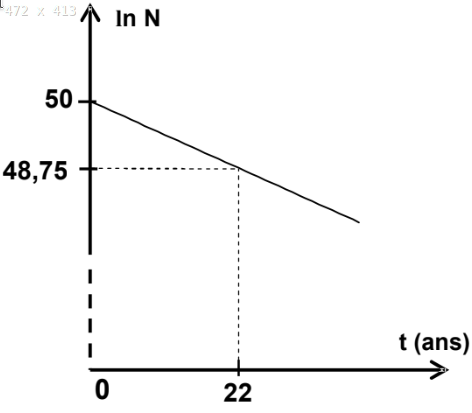
\includegraphics[width=0.25\textwidth]{./DesBeta.png}
  \end{center}
\end{wrapfigure}


\emph{L’énergie solaire provient de la réaction de fusion des noyaux d’hydrogène .Les physiciens
s’intéressent à produire l’énergie nucléaire à partir de la réaction de fusion des isotopes
d’hydrogène} : deutérium $^2_1H$ et tritium $^3_1H$ .

Données: Les masses en unité u: $m(^3_1H) = 3,01550u$ ; $m(^2_1H) = 2,01355 u$ ; $m(^4_2He) = 4,00150u$ ; $m(^1_0n) = 1,00866u$ ; $1u = 1,66.10^{-27}Kg = 931,5Mev.c^{-2}$
\vspace{0.4cm}

\textbf{1. La radioactivité $\beta^-$ du tritium}

Le nucléide tritium $^3_1H$ est radioactif $\beta^-$,
sa désintégration donne lieu à un isotope de
l’élément Hélium .

\begin{tabular}{c|l}

	1 & \makecell[l]{\textbf{1.1. }Ecrire l’équation de cette désintégration .}\\

	1 & \makecell[l]{\textbf{1.2. }On dispose d’un échantillon radioactif du
nucléide tritium $^3_1H$ contenant $N_0$ nucléides à \\l’instant t=0 .
Soit $N$ le nombre de nucléides tritium dans
l’échantillon à l’instant $t$ .
\\Le graphe de la figure1 représente les variations
de $ln(N)$ en fonction du temps t .
 \\ Déterminer la demi-vie $t_{1/2}$ du tritium . }\\
	\end{tabular}
  \vspace{0.4cm}

\textbf{2.Fusion nucléaire }

\textbf{2.1.} La courbe de la figure 2 représente les variations de l’opposé de l’énergie de liaison par
nucléon en fonction du nombre de nucléons A .

\begin{figure}[h]
\begin{center}
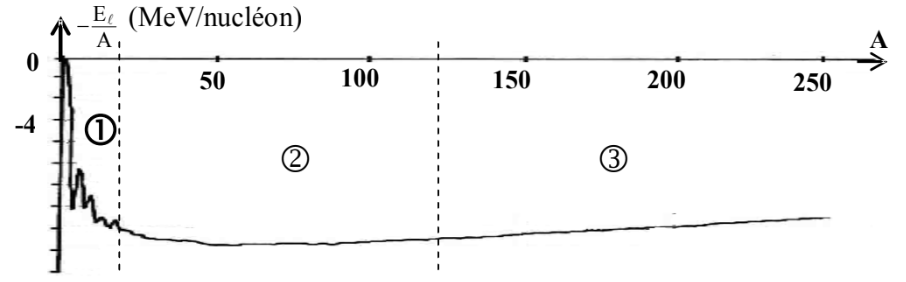
\includegraphics[width=13cm]{./segre_courbe.png}
	\end{center}
\end{figure}


	\begin{tabular}{c|l}

		1 & \makecell[l]{ Déterminer, parmi les intervalles 1 , 2 et 3 indiqués sur la figure 2, celui dans lequel les
nucléides \\sont susceptibles de subir des réactions de fusion . Justifier la réponse .}\\

		1 & \makecell[l]{\textbf{2.2 }Ecrire L’équation de la réaction de fusion des noyaux de deutérium et tritium }\\

		1,5 & \makecell[l]{\textbf{2.3 }On peut extraire 33mg de deutérium à partir de $1,0L$ de l’eau de mer .
Calculer, en MeV,\\la valeur absolue de l’énergie que l’on peut obtenir à partir de la réaction de
fusion du tritium \\et du deutérium extrait de $1 m^3$ de l’eau de mer .}\\
		\end{tabular}

\section*{Partie 2 : Datation par le carbone 14 \dotfill(7,5pts)}

Toutes les plantes absorbent le carbone $C$ qui se trouve dans l’atmosphère $(^{12}C$ et $^{14}C )$ à travers le dioxyde de
carbone de telle sorte que le rapport du nombre $N(^{14}C)_0$  des noyaux de carbone 14 à celui des noyaux du
carbone $N(C)_0$
dans les plantes reste constant durant leur vie : $\frac{ N(^{14}C)_0}{ N(C)_0} = 1,2.10^{-12}$

A partir de l’instant où la plante meurt, ce rapport commence à diminuer à cause de la désintégration du
carbone 14 qui est un isotope radioactif .

\textbf{Données}:
\begin{itemize}
  \item Demi-vie du carbone 14 : $t_{1/2} = 5730 ans$
  \item Masse molaire du carbone: M(C) = 12,0 g/mol
  \item Constante d’Avogadro : $N_A = 6,02.10^{23} mol^{-1}$
  \item $1an = 3,15.10^7$s.
  \item Le noyau du carbone 14 est radioactif $\beta^-$,sa désintégration donne un noyau $^A_ZY$.
\end{itemize}

1.La figure (1) donne une partie du diagramme de
Segri (Z,N) .


\begin{figure}[h]
\begin{center}
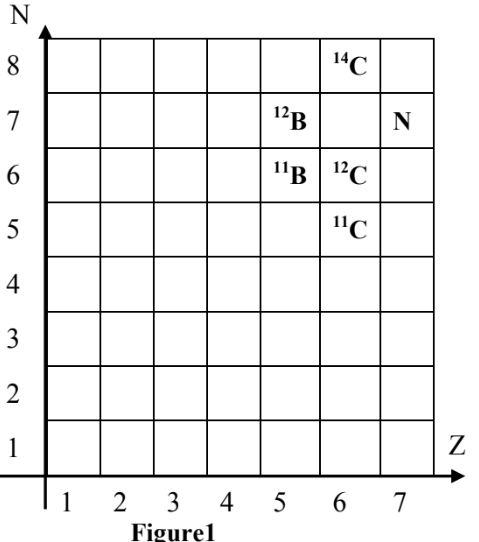
\includegraphics[width=7cm]{./diagramme_C_B.png}
	\end{center}
\end{figure}

\begin{tabular}{c|l}

 1 & \makecell[l]{\textbf{1.1 } Écrire l'équation complète de désintégration nucléaire du Carbone 14 puis représenter les deux \\noyaux père et fils
sur un digramme de Segré simplifié.}\\

 1 & \makecell[l]{\textbf{1.2 } Cette désintégration est-elle provoquée ou spontanée ? naturelle ou artificielle ?}\\

  1 & \makecell[l]{\textbf{1.3 }La désintégration du noyau du carbone $^{11}_6C$ donne un noyau de bore $^{A'}_{Z'}B$, \\Ecrire l’équation de cette transformation}\\
 \end{tabular}

 \vspace{0.4cm}
2. A l’aide du diagramme énergétique représenté
dans la figure (2) :


\begin{figure}[h]
\begin{center}
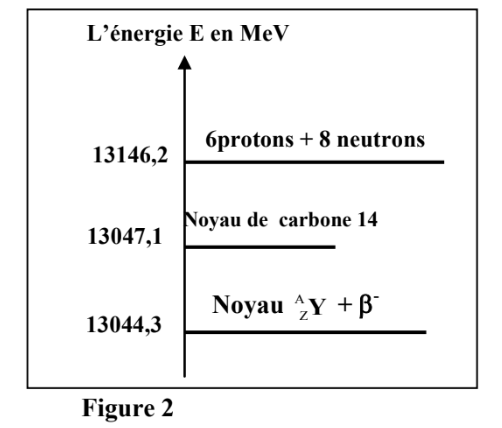
\includegraphics[width=7cm]{./desEquation.png}
	\end{center}
\end{figure}



\begin{tabular}{c|l}

 1 & \makecell[l]{\textbf{2.1 } Trouver l’énergie de liaison par nucléon du noyau de carbone 14 .}\\

 1 & \makecell[l]{\textbf{2.2 }}Trouver la valeur absolue de l’énergie produite
par la désintégration d’un noyau du carbone 14.\\
 \end{tabular}

3. On veut déterminer l’âge d’un morceau de bois
très ancien , pour cela on y prélève à un instant t
un échantillon de masse $m = 0,295g$ , on trouve
que cet échantillon donne $1,40$ désintégrations par
minute. On considère que ces désintégrations
proviennent uniquement du carbone 14 qui se trouve dans
l’échantillon étudié.

On prélève d’un arbre vivant un morceau de même masse que l’échantillon précédent $m = 0,295g$ , on
trouve que le pourcentage massique du carbone dans ce morceau est $51,2\%$

\begin{tabular}{c|l}

 1 & \makecell[l]{\textbf{3.1 } Calculer le nombre de noyaux du carbone C et le nombre de noyaux du carbone 14 dans \\le morceau qui a été prélevé de l’arbre vivant .}\\

 1,5 & \makecell[l]{\textbf{3.2 }Déterminer l’âge du morceau de bois ancien }\\
 \end{tabular}


\end{document}
